%\usepackage[T1]{fontenc}
%\usepackage[utf8]{inputenc}
%\usepackage{graphicx}

%!TEX ROOT=../diploma-thesis.tex

\chapter{Návrh}\label{ch:navrh}

V této kapitole budeme diskutovat návrh frameworku pro centrální správu
a automatickou distribuci business pravidel vyhovující požadavkům identifikovaným
v sekci~\ref{sec:implementation-requirements}. V předchozí kapitole~\ref{ch:reserse}
jsme prozkoumali architektury, které bychom mohli při návrhu využít, a shrnuli
jsme jejich výhody a nevýhody. Došli jsme k závěru, že alternativní přístup \gls{ADDA}
nám poskytne nejlepší aparát pro dosažení vytyčených cílů. Abychom ho mohli plně využít,
je nejprve potřeba formalizovat prostředí \gls{SOA} v rámci \gls{AOP}.

V rámci této kapitoly navrhneme vhodný způsob zachycení byznysových pravidel,
jejich uložení a organizaci v rámci systému. Bude potřeba vymyslet proces, jakým budou pravidla
automaticky distribuována. To bude vyžadovat vytvoření metamodelu, tedy struktury, která bude
sloužit k zachycení pravidel v paměti počítače.
Zároveň musíme navrhnout, jakým způsobem budou pravidla vyhodnocována při vykonávání byznysových operací.
Centrální správa pravidel vyžaduje vytyčení procesu, kterým bude možné administrovat
veškerá pravidla v systému s ohledem na zachování jejich konzisteního vykonávání.

\section{Formalizace architektury orientované na služby}

V kapitole~\ref{ch:analyza} jsme již identifikovali, jaké průřezové problémy, resp. aspekty,
jsou řešeny v informačních systémech. Dospěli jsme k závěru, že byznysová pravidla jsou
významným zástupcem těchto problémů. V sekci~\ref{sec:shortcomings} jsme shrnuli konkrétní
problémy byznysových pravidel, které konvenční přístup k návrhu a vývoji \gls{IS} neumí v rámci \gls{SOA} efektivně řešit.
Pro formalizaci \gls{SOA} do termínů \gls{AOP} musíme také identifikovat \textit{join-points},
ve kterých je možné aspekty v podobě byznysových pravidel aplikovat. Dále je potřeba určit podobu
\textit{advices}, popsat způsob jakým budou zachyceny \textit{pointcuts} a nakonec navrhnout proces
\textit{weavingu} pravidel.

\subsection{Join-points}

Při identifikování join-points budeme vycházet ze životního cyklu služby, který je znázorněn
na obrázku~\ref{fig:join-points}. První fází v životě instance služby je její inicializace,
konkrétně načtení aplikačního kontextu. V tomto bodě je potřeba získat veškerá pravidla, která
bude služba potřebovat ke své funkci.
Ve chvíli, kdy je inicializace hotova, vstupuje služba do fáze, ve které může přijímat požadavky
na vykonání byznysových operací. Pokud služba přijme takový požadavek, je nejprve nutno určit
byznysový kontext, a poté vyhodnotit veškeré \textit{preconditions}. Pokud jsou všechny předpoklady
pro spuštění operace splněny, může být vykonána. Po dokončení operace je nutno aplikovat relevantní
post-conditions.

\begin{figure}
    \centering
    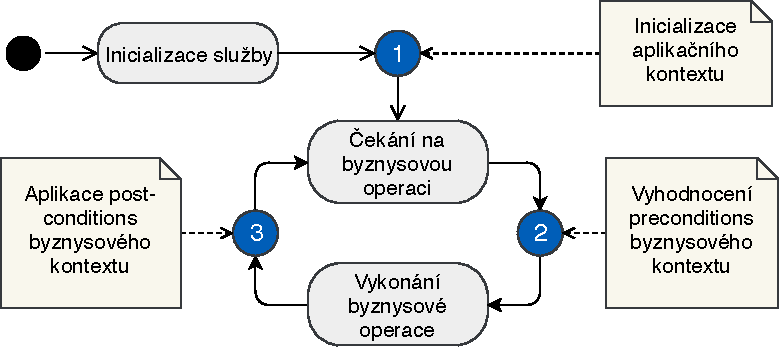
\includegraphics[keepaspectratio=true, width=0.8\linewidth]{figures/join-points.pdf}
    \caption{Diagram životn\'{\i}ho cyklu služby a identifikovan\'ych join-pointů}
    \label{fig:join-points}
\end{figure}

Identifikované join-points tedy jsou:

\benum[label=\circledarabic]
\item\label{itm:initialization} Inicializace instance služby
\item\label{itm:before} Volání byznysové operace
\item\label{itm:after} Dokončení byznysové operace
\eenum

\subsection{Pointcuts}

V join-pointu~\ref{itm:initialization} by služba měla načíst všechna byznysová pravidla, která
bude potřebovat ke své činnosti, a nejsou pro ni lokálně dostupná. Služba tedy musí zjistit,
která pravidla je potřeba získat, a následně si je vyžádat od ostatních služeb.
V join-pointech~\ref{itm:before}~a~\ref{itm:after} musejí být aplikována byznysová pravidla každého
kontextu vztahujícího se k dané operaci.

Nyní je potřeba se zamyslet, jakým způsobem budou selektory join-pointů pro jednotlivá pravidla zapsány.
Pokud bychom chtěli u každého byznysového pravidla zapsat, ke kterým byznysovým operacím se vztahuje,
museli bychom předem znát seznam veškerých byznysových operací implementovaných v celém systému. Pokud si
představíme příklad ze sekce~\ref{sec:shortcomings}, musela by služba implementující vystavování
faktur předem vědět o všech případech, kde bude potřeba validovat validační adresu, aby tato místa mohla
adresovat. To ovšem není příliš vhodné řešení.

\lstinputlisting[
caption={Ukázka zápisu validačních pravidel pomocí anotací v jazyku Java},
label={lst:jsr303},
language=Java,
%frame=single,
float,
floatplacement=t
]
{code/jsr303.java}

Lepším způsobem by bylo nechat kontrolu na byznysových operacích. Ty by si mohly samy vyžádat
byznysová pravidla, která potřebují. Tento koncept je využíván například standardem \gls{JSR}
303~\cite{bernard2009jsr}, který umožňuje validovat data byznysových objektů vstupujících do
byznysových operací pomocí anotací atributů těchto objektů. Příklad validačních anotací můžeme vidět ve zdrojovém kódu~\ref{lst:jsr303},
kde je pomocí anotace \code{$@$NotNull} zajištěno, že fakturační adresa bude mít vyplněná všechna
náležitá pole. V našem kontextu se tedy jedná o paralelu preconditions. Místo toho, abychom u
validačního pravidla \code{$@$NotNull} vypisovali všechna místa v kódu, kde má být použito,
využijeme na těchto místech jeho anotaci. V našem případě by podobným způsobem každá byznysová operace, která
by využívala pravidla pro validaci fakturační adresy, mohla specifikovat, že toto pravidlo bude využívat.

Toto řešení nám však neposkytuje možnost dynamicky při běhu programu změnit sadu byzynsových pravidel,
které mají být aplikovány na byzynsovou operaci. Museli bychom konfiguraci toho, která pravidla
budou aplikována na kterou operaci, přesunout do jakési externí dynamické konfigurace. To by ale významně
snížilo přehlednost kódu. Vhodným kompromisem by mohl být koncept byznysového kontextu, který
zapouzdřuje byznysová pravidla, a byznysová operace se na něj může explicitně odkázat. Byznysový kontext
by přitom mohl být dynamicky změněn za běhu programu.

Sdílení pravidel mezi byznysovými kontexty, potažmo byznysovými operacemi a mezi jednotlivými službami,
by mohlo být realizováno pomocí dědičnosti kontextů. Každý kontext, který by potřeboval validovat fakturační
adresu, by tak mohl pouze dědit od kontextu vytváření faktury. Na obrázku~\ref{fig:context-extension} můžeme vidět,
jak by takový případ mohl vypadat. Kontext vytváření objednávky dědí od kontextu vytváření faktury
a sdílí tak jeho byznysová pravidla. Byznysové operace se odkazují na byznysové kontexty, které mají
být při jejich vykonávání použity. Jak můžeme vidět, před spuštěním a po dokončení operace vytváření
objednávky jsou aplikována pravidla obou kontextů, zatímco při vytváření faktury jsou zohledněna
pouze pravidla jednoho kontextu.

\begin{figure}
    \centering
    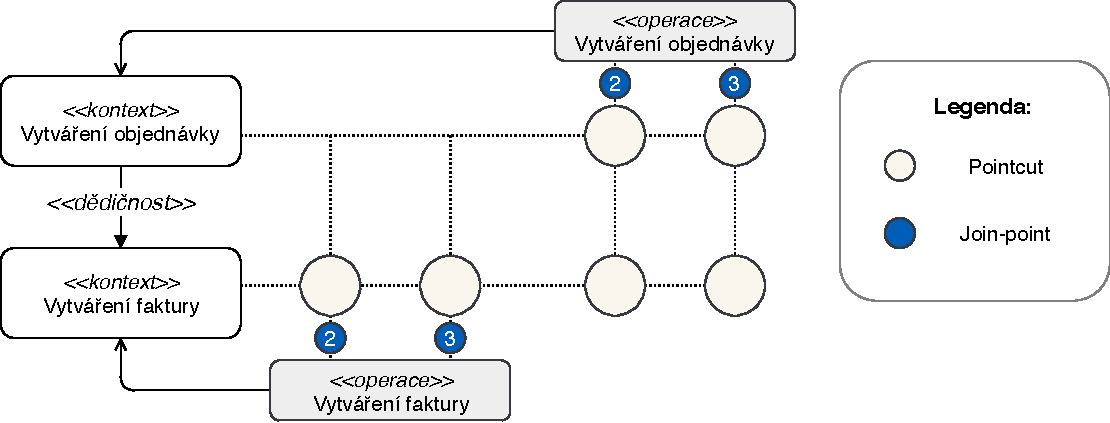
\includegraphics[keepaspectratio=true, width=1\linewidth]{figures/context-extension.pdf}
    \caption{Diagram znázorňující dědičnost kontextů ve vztahu k join-pointům a pointcuts}
    \label{fig:context-extension}
\end{figure}

\subsection{Advices}

V případě join-pointu~\ref{itm:initialization} se za advice dá považovat repretenzace byznysového
kontextu přenášeného mezi službami. Naopak v join-pointech~\ref{itm:before}~a~\ref{itm:after}
je přidanou funkcionalitou vyhodnocování preconditions nad aplikačním kontextem, resp. aplikování
post-conditions na návratovou hodnotu operace.

\subsection{Weaving}

Weaving v případě join-pointu~\ref{itm:initialization} provádí komponenta frameworku, která
analyzuje lokálně dostupná pravidla služby, vyhodnotí, která pravidla je potřeba stáhnout,
a vyžádá tato pravidla od příslušných služeb.

V případě join-pointů~\ref{itm:before}~a~\ref{itm:after} se o weaving postará speciální aspect weaver.
Ten zachytí volání byznysové operace a získá informace o aktuálním stavu aplikačního kontextu.
Následně zjistí, který byznysový kontext má být aplikován, shromaždí všechny preconditions
a každou z nich vyhodnotí. Pokud některá precondition není splněna, byznysová operace je zastavena
a je vyhozena výjimka, na kterou musí služba reagovat. V opačném případě je kontrola vrácena zpět
službě, která vykoná byznysovou operaci. Po jejím dokončení opět přichází na řadu aspect weaver,
který zachytí výstup byznysové operace a aplikuje post-conditions daného byznysového kontextu.
Proces weavingu je zachycen na obrázku~\ref{fig:business-rules-weaver}.

\begin{figure}
    \centering
    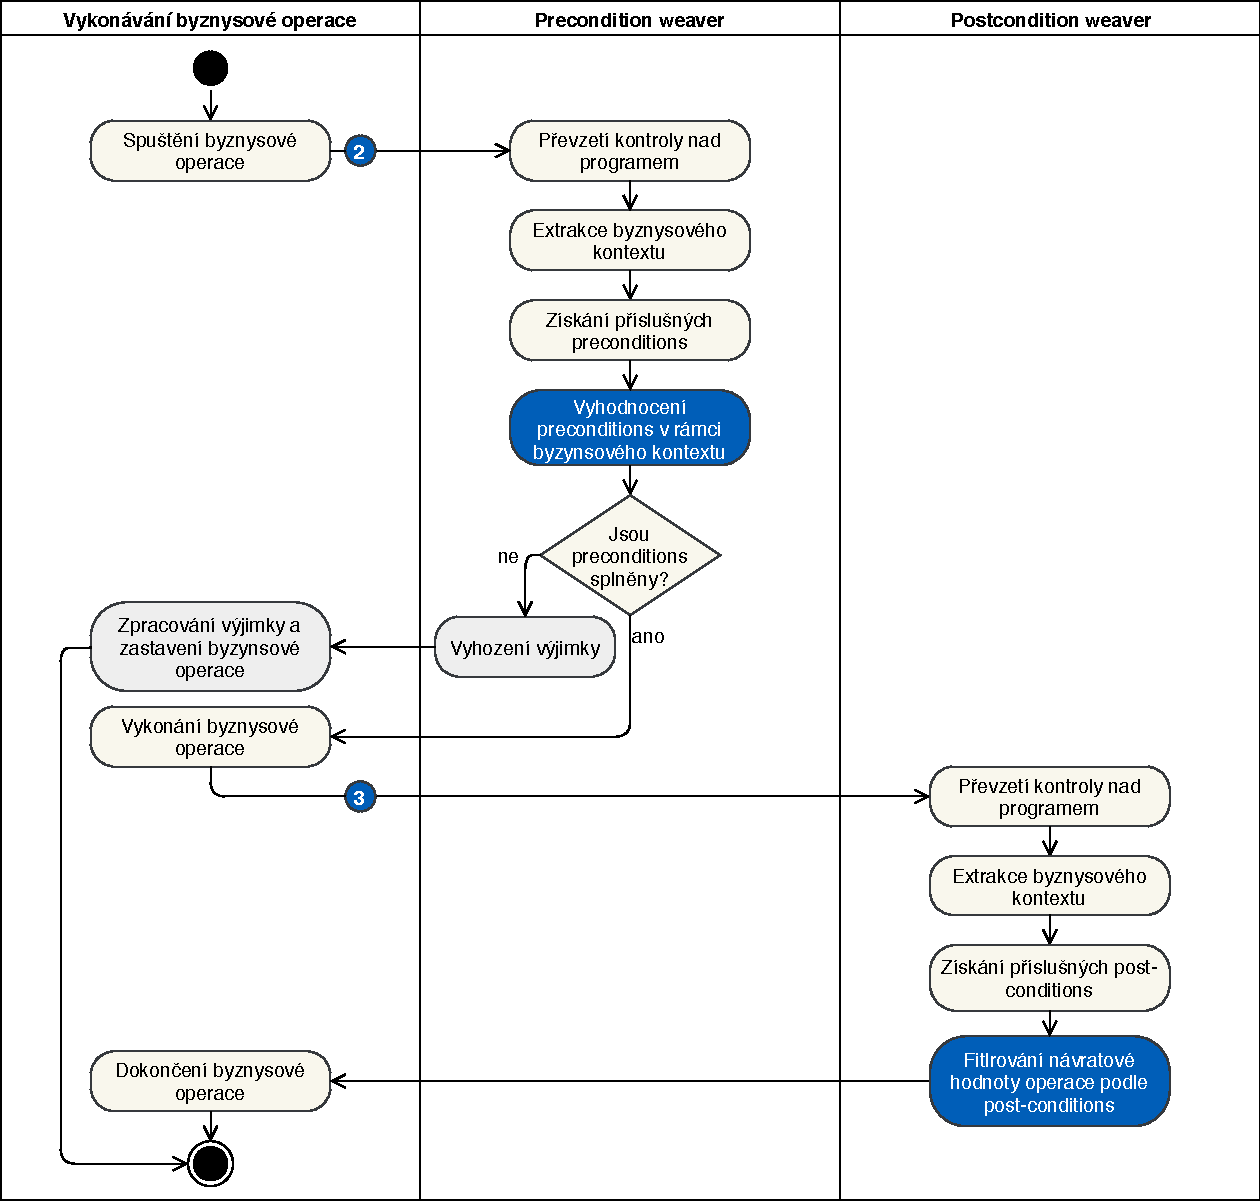
\includegraphics[keepaspectratio=true, width=0.8\linewidth]{figures/business-rules-weaver.pdf}
    \caption{Diagram aktivit weaverů byznysov\'ych pravidel}
    \label{fig:business-rules-weaver}
\end{figure} % TODO: popsat

\section{Dědičnost byznysových kontextů}\label{sec:context-inheritance}

V předchozím textu jsme představili kontext dědičnosti byznysových kontextů. Ten funguje tak,
že libovolný kontext může rozšiřovat libovolné množství jiných kontextů, a sdílet jejich
byznysová pravidla, tedy jejich preconditions a post-conditions. Byznysové operace
pak mohou samy určit, který byznysový kontext se k ním váže. Budeme-li chtít tento
koncept využít, musíme však vyřešit několik otázek, které přináší.

Pokud bychom mapovali byznysové kontexty a byznysové operace jedna ku jedné, mohla by
nastat situace, kdy chceme využít pouze nějaká byznysová pravidla jiného kontextu,
ale ne všecha. Příkladem může být proces vytváření objednávky a proces registrace uživatele.
Při vytváření objednávky chceme zaslat uživateli potvrzující mail, a proto potřebujeme, aby
měl vyplněnou e-mailovou adresu. Zároveň chceme, aby byl uživatel při vytváření objednávky přihlášený.
Při registraci uživatele bychom mohli rozšířit kontext vytváření objednávky, ovšem nechceme využít pravidlo
vyžadující přihlášení uživatele. Tuto situaci lze vyřešit tak, že rozvolníme vztah mezi kontexty a operacemi
a umožníme využívat tzv. \textit{abstraktní kontexty} \textendash\xspace tedy takové kontexty, které
přímo nevyužívá žádná byznysová operace. V našem příkladu bychom mohli tedy pravidlo vyžadující vyplnění
emailové adresy vyčlenit do abstraktního kontextu, ze kterého by dědil jak kontext vytváření uživatele,
tak kontext vytváření objednávky. Situace je znázorněna na obrázku~\ref{fig:abstract-context}.

\begin{figure}
    \centering
    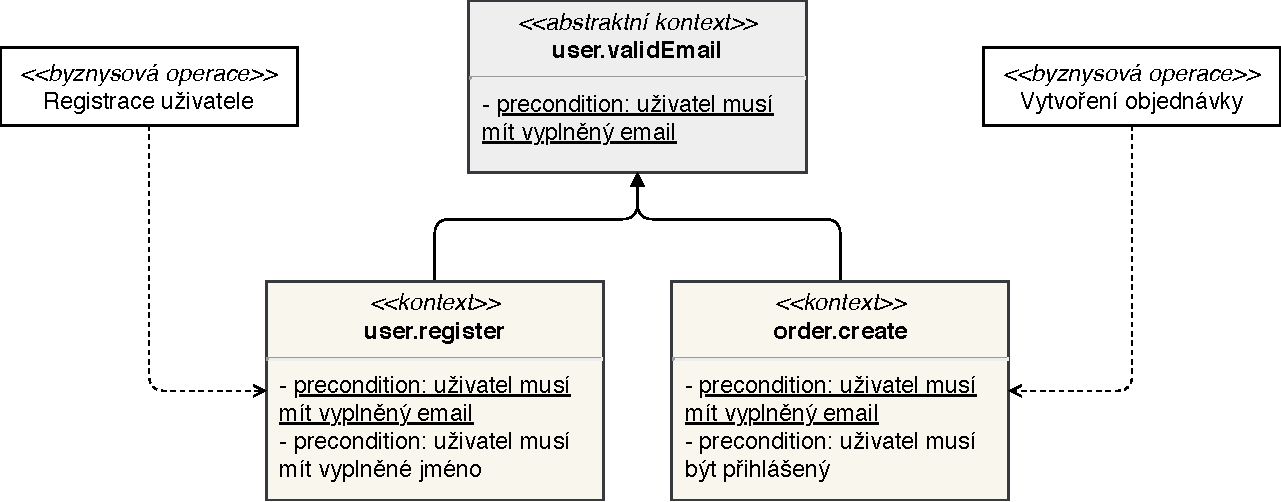
\includegraphics[keepaspectratio=true, width=1\linewidth]{figures/abstract-context.pdf}
    \caption{Diagram konceptu abstraktního byznysového kontextu}
    \label{fig:abstract-context}
\end{figure}

Dalším problémem je kruhová závislost kontextů, která nastává, když kontext A dědí od kontextu B,
a ten opět dědí od kontextu A. Pokud tato situace nastane, nemůžeme ji z hlediska frameworku vyřešit.
Je tedy nutné, aby byznysové kontexty systému využívajícího námi navrhovaný framework neobsahovaly cyklus.
K zajištění této skutečnosti by mohl sloužit validátor vestavěný do nástroje pro správu byznysových kontextů.

Kvůli vícenásobné dědičnosti může nastat problém, kdy jeden kontext zdědí více stejných pravidel z
různých zdrojů. Představme si, že kontext D dědí od kontextů B a C, přičemž kontexty B a C dědí
od kontextu A. Kontext D pak zdědí pravidla kontextu A dvakrát. Tomu lze předejít tak, že
každé pravidlo bude mít unikátní identifikátor v rámci celého systému. V případě, že kontext
získá dvě pravidla se stejným identifikátorem, vybere si jen jedno z nich a druhé může zahodit, protože
jsou identická. Zajištění unikátního identifikátoru můžeme vynutit díky nástroji pro centrální
administraci byznysových pravidel, která je součástí navrhovaného frameworku.

Nakonec bychom měli zvážit problém, kdy kontext kvůli dědičnosti získá takovou množinu
preconditions, která nebude nikdy splnitelná. Příklad je velmi jednoduchý \textendash\xspace
pokud jedna precondition vyžaduje příhlášení uživatele a druhá precondition naopak požaduje,
aby uživatel nebyl přihlášen, nemůže nastat situace, kdy budou obě preconditions uspokojeny.
Takovéto stavy by měl primárně hlídat administrátor či architekt systému, nicméně můžeme
jeho práci usnadnit díky nástroji pro centrální administraci kontextů.

\section{Logické výrazy byznysových pravidel}

V sekci~\ref{sec:business-rules} jsme analyzovali byznysová pravidla a jedním z
našich zjištění bylo, že pravidla obsahují logické podmínky, které je
potřeba vyhodnocovat. V případě preconditions je to ověření podmínky,
která musí být platná před spuštěním byznysové operace. V případě post-conditions,
kdy chceme filtrovat návratovou hodnotu byzynsové operace, nemusíme logickou podmínku
potřebovat vždy. Může ale nastat moment, kdy chceme filtrovat hodnotu pouze pokud je
splněna nějaká podmínka \textendash\xspace například pokud uživatel není administrátorem.

\begin{figure}
    \centering
    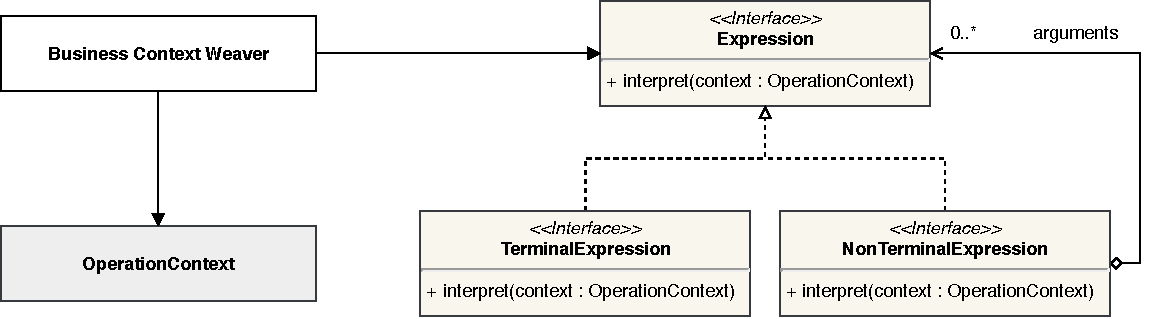
\includegraphics[keepaspectratio=true, width=1\linewidth]{figures/expression.pdf}
    \caption{Diagram tříd popisující použití vzoru Intepreter pro vyhodnocování logických výrazů}
    \label{fig:expression}
\end{figure}

Vyhodnocování logických výrazů byznysových pravidel bude prováděno naším frameworkem
při weavingu byznysových kontextů. K tomuto účelu je velmi vhodný návrhový vzor
\textit{Interpreter}~\cite{fowler2002patterns}. Základní myšlenkou tohoto vzoru je
interpretace jazyka, kdy každý jeho výraz (z anglického \textit{expression}) je reprezentován
samostatným objektem, který přebírá zodpovědnost za správnou interpretaci daného výrazu.
Logické výrazy tvoří orientovaný acyklický graf (\gls{DAG}), tzv. \textit{derivační strom},
a rozdělují se na tzv. \textit{terminály} a \textit{neterminály}~\cite{melichar2003jazyky}. Terminál znamená,
že z daného výrazu již nevychází žádná hrana do jiného výrazu. Neterminál je opak terminálu.
Na obrázku~\ref{fig:expression} můžeme vidět použití vzoru interpreter pro náš účel.
Můžeme si také všimnout, že strom výrazů opisuje návrhový vzor \textit{Composite}~\cite{fowler2002patterns}.

V rámci vzoru Interpreter si dále můžeme všimnout toho, že vyhodnocované výrazy mají přístup
k objektu \code{OperationContext}. V něm jsou držena veškerá data, která jsou pro interpretaci
výrazu potřebná. Jednotlivé výrazy se tedy mohou odkazovat na proměnné či konstanty obsažené
v tomto kontextu. Pokud bude uživatel frameworku potřebovat rozšířit funkcionalitu pravidel,
mohly by se mu hodit i speciální funkce, které by si mohl do operačního kontextu zadefinovat.

V rámci této kapitoly bychom bychom měli navrhnout i základní sadu výrazů, které budou
sloužit pro zápis byznysových pravidel. Kromě základních logických operací jako je
\code{and}, \code{or}, \code{equals} a \code{negate} budeme potřebovat i výraz,
který získá hodnotu proměnné či konstanty z kontextu. Pokud bude v proměnné uložen
objekt, bude potřeba přistupovat i k jeho veřejným atributům, což bude vyžadovat další
speciální výraz. Uživatel taky potřebuje možnost otestovat, zda je v odkazované proměnné
hodnota. K tomu může sloužit výrat \code{IsNotNull}, který ověří proměnnou libovolného
typu na přítomnost hodnoty, a výraz \code{IsNotBlank}, který ověří, zda je v proměnné řetězec
nenulové délky. Některé případy použití mohou vyžadovat vložení konstantní hodnoty přímo do byznysového
pravidla \textendash\xspace k tomuto účel by mohl sloužit speciální terminál \code{Constant}.
Pro zvýšený komfort můžeme do frameworku přidat i podporu základních matematických operací,
jako je sčítání, odečítání, násobení a dělení. Pro volání funkcí definovaných
v operačním kontextu je zapotřebí další speciální výraz. V jeho případě je nutno
dbát na to, že funkce může přijímat libovolný počet argumentů. Protože volaná funkce může potřebovat
přistupovat k operačnímu kontextu, musejí být argumenty také interpretovány naším frameworkem.
Bohužel nemůžeme u uživatelem definovaných funkcí ověřit, že bude při volání byznysového pravidla odpovídat
počet a typ argumentů. Toto si tedy bude muset uživatel frameworku zajistit sám.
Přehled všech výrazů, které bude framework podporovat, je v tabulce~\ref{tbl:expressions},

\afterpage{%
\clearpage% Flush earlier floats (otherwise order might not be correct)
\thispagestyle{empty}% empty page style (?)
\begin{landscape}
\begin{table}
    \centering
    \begin{tabular}{ l l l c c }
        \hline
        \textbf{Název} & \textbf{Argumenty} & \textbf{Atributy} & \textbf{Návratový typ} & \textbf{Typ výrazu} \\ \hline \hline
        \textbf{Constant} & - & Hodnota a typ konstanty & \code{?} & Terminál \\
        \textbf{FunctionCall} & Libovolný počet argumentů & Návratový typ funkce & \code{?} & Terminál \\
        \textbf{IsNotNull} & Jeden argument libovolného typu & - & \code{BOOL} & Neterminál \\
        \textbf{IsNotBlank} & Jeden argument typu \code{STRING} & - & \code{BOOL} & Neterminál \\
        \textbf{LogicalAnd} & 2 argumenty typu \code{BOOL} & - & \code{BOOL} & Neterminál \\
        \textbf{LogicalEquals} & 2 argumenty libovolného typu & - & \code{BOOL} & Neterminál \\
        \textbf{LogicalNegate} & 1 argument typu \code{BOOL} & - & \code{BOOL} & Neterminál \\
        \textbf{LogicalOr} & 2 argumenty typu \code{BOOL} & - & \code{BOOL} & Neterminál \\
        \textbf{NumericAdd} & 2 argumenty typu \code{NUMBER} & - & \code{NUMBER} & Neterminál \\
        \textbf{NumericSubtract} & 2 argumenty typu \code{NUMBER} & - & \code{NUMBER} & Neterminál \\
        \textbf{NumericMultiply} & 2 argumenty typu \code{NUMBER} & - & \code{NUMBER} & Neterminál \\
        \textbf{NumericDivide} & 2 argumenty typu \code{NUMBER} & - & \code{NUMBER} & Neterminál \\
        \textbf{ObjectReference} & - & Název objektu a název a typ proměnné & \code{?} & Terminál \\
        \textbf{VariableReference} & - & Název a typ proměnné & \code{?} & Terminál \\
        \hline
    \end{tabular}
    \caption{Přehled výrazů pro zápis byznysového pravidla}
    \label{tbl:expressions}
\end{table}
\end{landscape}
\clearpage% Flush page
}

\goal{Typované výrazy}
Musíme mít na paměti, že konstanty a proměnné mohou nabývat různých hodnot rozdílného typu.
Pokud navrhujeme framework, který má sloužit pro více platforem,
existuje možnost, že některý z podporovaných jazyků bude využívat typový systém.
Pro ulehčení implementace tedy musíme k logickým výrazum uložit i
informace o typu jejich argumentů a jejich návratové hodnoty.
Díky tomu bude možné framework rozšířit o typovou kontrolu, což přinese menší náchylnost
k sémantickým chybám v zápisu pravidla. Výraz byznysového pravidla
může nabývat logických hodnot, může vracet číslo, textový řetězec a také objekt. Musíme také
počítat s tím, že výraz nevrací žádnou hodnotu. Je nutno podotknout, že vzhledem k povaze
byznysových pravidel musí kořen pravidla vždy vracet logickou hodnotu. Následuje výčet typů,
kterých mohou výrazy nabývat.

\begin{itemize}
    \item \code{BOOL} je logický typ, který nabývá hodnoty \code{true} a \code{false}.
    \item \code{NUMBER} je reálné číslo zapsáno ve tvaru s desetinnou tečkou a neomezeným počtem číslic.
    \item \code{OBJECT} je objekt libovolného typu.
    \item \code{STRING} je textový řetězec.
    \item \code{VOID} je pseudotyp značící, že výraz nemá návratovou hodnotu.
\end{itemize}

\goal{Atributy pravidel}
Kromě argumentů neterminálů je v některých případech potřeba k výrazu uložit i dodatečné informace.
Nazývejme je \textit{atributy}. Jedním z atributů je typ návratové hotnoty výrazu, pokud není přímo implikována.
V případě výrazu \code{Constant} je potřeba uložit hodnotu a typ konstanty. Reference na proměnnou
musí obsahovat její název a typ, reference na pole objektu navíc musí obsahovat název odkazovaného pole.
Volání funkce musí obsahovat její název a návratový typ.

\begin{figure}
    \centering
    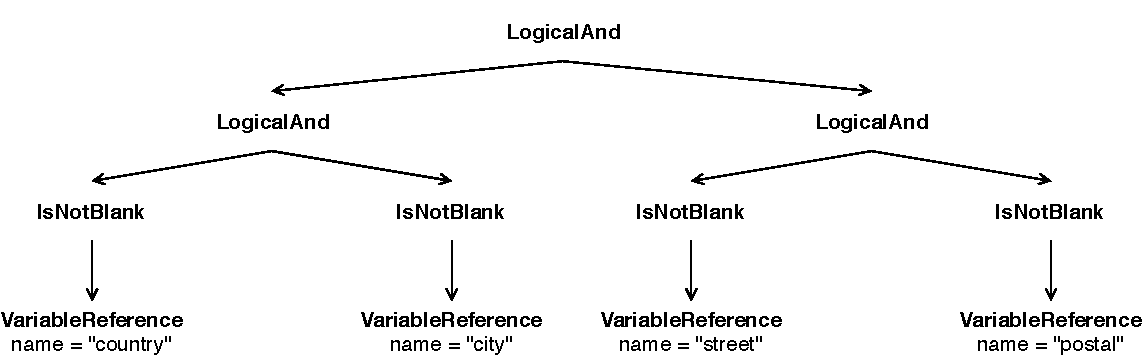
\includegraphics[keepaspectratio=true, width=1\linewidth]{figures/simple-rule.pdf}
    \caption{Syntaktický strom jednoduchého validačního pravidla}
    \label{fig:simple-rule}
\end{figure}

\goal{Příklad AST pravidla}
Na obrázku~\ref{fig:simple-rule} můžeme vidět syntaktický strom, který zachycuje jednoduché
validační pravidlo validující fakturační adresu. Jedná se o ekvivalent validačních pravidel
zachycených ve zdrojovém kódu~\ref{lst:jsr303} pomocí anotací standardu \gls{JSR} 303.
Pravidlo je tvořeno čtyřmi teminály, které se odkazují na proměnné operačního kontextu \code{country},
\code{city}, \code{street} a \code{postal}. Každá z těchto proměnných je argumentem validačního výrazu
\code{IsNotBlank}. Tento výraz vrací hodnotu \code{true}, pokud jeho argumentem je řetězec, který obsahuje
alespoň jeden znak. Jednotlivé validace jsou poté spojeny pomocí binárního výrazu \code{LogicalAnd},
který vrací hodnotu \code{true} tehdy a pouze tehdy, když oba jeho argumenty mají hodnotu \code{true}.
Pro přehlednost jsme do diagramu nezanášely návratové typy výrazů.

\section{Filtrování návratových hodnot byznysové operace}

Při aplikování post-conditions je potřeba navrhnout, jakým způsobem bude probíhat filtrování
návratové hodnoty byznysové operace. Návratovou hodnotou může být proměnná obsahující jednoduchou
hodnotu, jako je číslo nebo text, objekt, či kolekci hodnot nebo objektů. Filtrování jednoduchých
hodnot nemá význam, protože by to znamenalo, že byznysová operace nevrátí žádnou hodnotu, ačkoliv
s tím kód sytému může počítat. Pokud bude vývojář systému chtít tuto možnost opravdu použít, může
jednoduchou návratovou hodnotu zabalit do objektu, který ji bude přenášet.
V případě návratové hodnoty v podobě objektu pak můžeme požadovat filtrování některých jeho atributů,
například můžeme chtít při zobrazování uživatelského profilu filtrovat e-mailovou adresu uživatele,
pokud uživatel není administrátor. V případě kolekce můžeme požadovat, aby byly některé její prvky odstraněny,
například nechceme zobrazit objednávky, které uživateli nepatří. Pokud se v kolekci nachází objekty, můžeme
také požadovat, aby byly zakryty atributy jednotlivých objektů \textendash\xspace analogie na filtrování e-mailových
adres v kolekci více uživatelů. Itentifikovanými typy post-conditions tedy jsou:

\begin{itemize}
    \item \code{FILTER\_OBJECT\_FIELD} filtruje atribut objektu, který je výstupem operace.
    \item \code{FILTER\_LIST\_OF\_OBJECTS} filtruje objekty v kolekci, která je výstupem operace.
    \item \code{FILTER\_LIST\_OF\_OBJECTS\_FIELDS} filtruje atributy objektů v kolekci, která je výstupem operace.
\end{itemize}

V tuto chvíli je potřeba zavést konvenci, která bude říkat, kdy bude návratová hodnota
vyfiltrována, konkrétně zda to bude při splnění či nesplnění podmínky post-condition.
V textu výše jsme uváděli, že post-condition bude aplikována, pokud je podmínka splněna.
Držme se tedy tohoto značení.

\section{Metamodel byznysového kontextu}\label{sec:metamodel}

Když nyní známe způsob, jakým zachytíme podmínky byznysových pravidel, můžeme
navrhnout kompletní model byznysových pravidel, potažmo byznysových kontextů.
Kromě samotných logických výrazů je potřeba také ukládat informace o tom, zda
se jedná o precondition nebo post-condition, a identifikátor pravidla. Post-condition
navíc potřebuje uložit informaci o jejím typu a názvu. Jak jsme již v předchozím
textu psali, pravidla budou uskupována do byznysových kontextů, z nichž každý
má svůj unikátní identifikátor skládající se z prefixu a samotného jména a také
drží informaci o tom, od kterých ostatních kontextů dědí.
Diagram tříd navrženého kontextu je znázorněn na obrázku~\ref{fig:business-context-metamodel}.

\begin{figure}
    \centering
    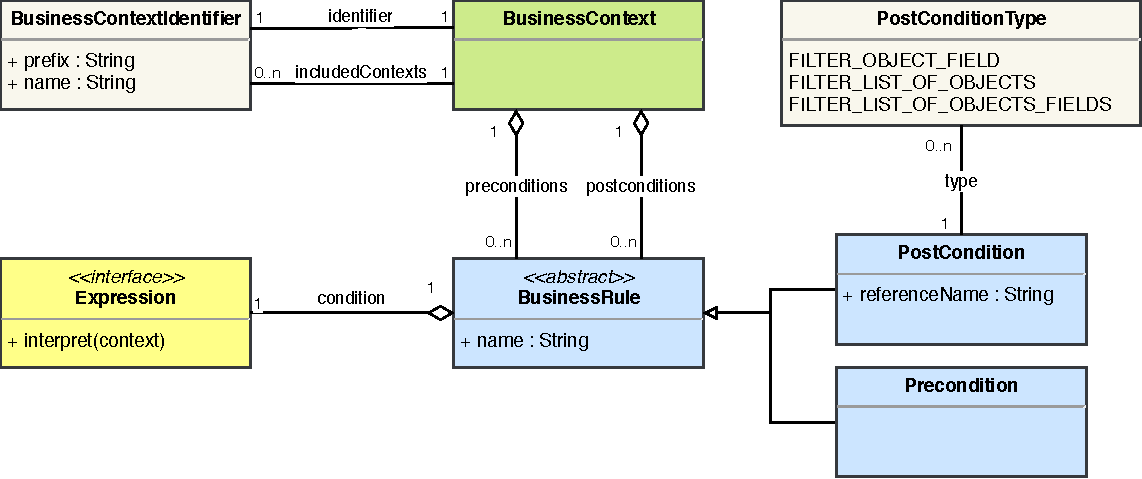
\includegraphics[keepaspectratio=true, width=\linewidth]{figures/business-context-metamodel.pdf}
    \caption{Diagram tř\'{\i}d metamodelu byznysového kontextu}
    \label{fig:business-context-metamodel}
\end{figure}

\section{Popis byznysových pravidel pomocí \gls{DSL}}

Př\'{\i}stup \gls{ADDA} doporučuje popsat byznysová pravidla pomoc\'{\i}
vlastn\'{\i}ho, na m\'{\i}ru šitého, doménově specifického jazyka~\cite{cemus2015automated}.
V našem př\'{\i}padě můžeme jazykem \gls{DSL} popsat kompletně i cel\'y
byznysov\'y kontext.

V sekci~\ref{sec:business-rule-dsl} jsme zjistili, že ačkoliv jsou nástroje Drools a JetBrains
MPS velmi silnými aparáty, jejich vlastnosti nejsou plně vhodné pro řešení problému
centrální administrace a automatické distribuce byznysových pravidel.
Můžeme jít cestou volby co nejvhodnějšího jazyka pro každou platformu, kterou chceme
využívat pro naše účely, a implementace adapterů pro tyto jazyky, které transformují
dané \gls{DSL} do metamodelu. Vzhledem k různým vlastnostem těchto jazyků by ale takový
přístup byl suboptimální, museli bychom totiž zohlednit \uv{nejmenší společný jmenovatel}
\textendash\xspace tedy zápis kontextu by byl limitován sjednocením všech nedostatků těchto jazyků.

Na tomto místě bychom měli specifikovat, jak by \gls{DSL} popisující byznysový kontext mělo vypadat.
\gls{DSL} popisující byznysový kontext by mělo umožňovat zachytit identifikátor, seznam kontextů,
které rozšiřuje, a poté jednotlivá pravidla, tedy preconditions a post-conditions. Každé byznysové pravidlo musí
mít svůj vlastní identifikátor a podmínku vyjádřenou logickým výrazem, který jsme detailně rozebrali
v předchozím textu. Post-condition musí navíc obsahovat popis typu a kromě typu \code{FILTER\_LIST\_OF\_OBJECTS} je
také potřeba popsat název pole, které má být v objektu filtrováno.

\begin{figure}
    \centering
    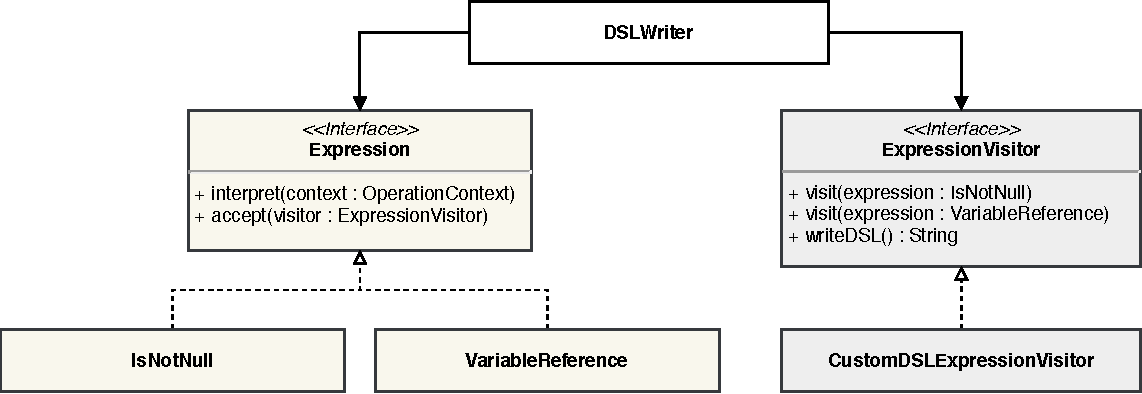
\includegraphics[keepaspectratio=true, width=1\linewidth]{figures/expression-visitor.pdf}
    \caption{Diagram tříd popisující využití vzoru Visitor pro zápis logických výrazů v \gls{DSL}}
    \label{fig:expression-visitor}
\end{figure}

Pro efektivní využití \gls{DSL} musíme také navrhnout způsob, jakým bude
popis byznysového kontextu a jeho pravidel převáděn do metamodelu a vice versa.
Pro načtení kontextu z \gls{DSL} může sloužit
návrhový vzor a \textit{parser}~\cite{scott2000programming}. Jejich volba se bude
odvijet od zvoleného \gls{DSL}.
Pro uložení kontextu do \gls{DSL}, aby ho mohl vývojář či administrátor
systému upravovat, je vzhledem ke zvolené reprezentaci a popisu logických
výrazů derivačním stromem ideální volbou návrhový vzor \textit{Visitor}~\cite{fowler2002patterns}.
Ten umožní elegantně převádět libovolně složité logické výrazy pomocí metody
\textit{double-dispatch}. Jeho volbou zároveň umožníme rozšiřitelnost frameworku
pro libovolné \gls{DSL} \textendash\xspace bude stačit implementovat konkrétní
visitor pro zvolený jazyk, aniž by bylo nutno zasahovat přímo do implementace frameworku.
Princip použití vzoru Visitor je znázorněn na obrázku~\ref{fig:expression-visitor}.

Samotný návrh a implementace kvalitního \gls{DSL} splňující naše požadavky není předmětem
této práce a je bohužel mimo její rozsah. Nicméně, v tuto chvíli můžeme pokračovat v návrhu
frameworku, protože známe všechny potřebné detaily popisu byznysových kontextů. Framework je
navíc na konkrétním \gls{DSL} nezávislý. Uživatelé frameworku dokonce mohou sestrojit
\gls{DSL} na míru potřebě svého systému a díky tomu dosáhnou maximálního komfortu při jeho vývoji.

\section{Organizace byznysových pravidel}

Předpokládáme, že každá služba má lokálně uložen popis byznysových kontextů, které se sémanticky vztahují
k její doméně. Jak jsme již nastínili v sekci~\ref{sec:shortcomings}, služba při výkonu jedné byznysové
operace může potřebovat aplikovat byznysová pravidla, která jsou aplikována také při výkonu jiné byznysové operace
v jiné službě \textendash\xspace tedy patří do byznysového kontextu jiné služby. Abychom mohli lépe
určit, kde jsou jednotlivá pravidla, potažmo jednotlivé kontexty definovány, přidáme do identifikátoru kontextu
tzv. \textit{prefix}. Jeden prefix pak bude spravován výhradně jednou službou a podle toho poznáme,
kde v systému jednotlivé kontexty hledat. Například kontexty služby spravující objednávky budou
označeny prefixem \code{order}, zatímco kontexty služby zajišťující fakturaci budou označeny prefixem \code{billing}.
Může nastat situace, kdy jedna služba bude spravovat více prefixů \textendash\xspace to však ničemu nevadí.

\subsection{Registr byznysových kontextů}

Cílem našeho přístupu je soustředit byznysové kontexty na jedno místo, ze kterého budou
automaticky distribuovány. Pro tento účel využijeme komponentu, která bude mít
za úkol kontexty načítat z \gls{DSL} do metamodelu, načítat lokálně nedostupné kontexty
z ostatních služeb a načtené kontexty uchovávat pro použití při weavingu. Tuto komponentu
budeme nazývat registr byzynsových kontextů (\code{BusinessContextRegistry}).
Každá služba pak bude disponovat svým registrem. Při inicializaci kontextů spolu budou registry komunikovat
a vyměňovat si sdílené kontexty.

\subsection{Uložení kontextů}

Byznysové kontexty popsané pomocí \gls{DSL} mohou být v příslušné službě uložena v souborech na disku či v
databázi. Navrhovaný framework by na způsobu uložení neměl být závislý a o potřebné kroky
pro načtení či případně uložení kontextu se postará konkrétní implementace. Pro tento účel
je tedy vhodné, aby registr pracoval s nekonkrétními rozhraními, na jejichž implementaci
nebude nijak záviset.

\section{Inicializace byznysových kontextů}
Při inicializaci služby je potřeba načíst všechny byznysové kontexty, které bude služba
pro svůj běh potřebovat. Mohli bychom argumentovat, že načítat příslušný kontext by šlo
až ve chvíli, kdy je opravdu zavolána byznysová operace. Kontext bychom pak mohli uložit
do paměti, aby se nemusel načítat při dalším spuštění operace. Toto řešení by rozprostřelo
latenci při inicializaci služby mezi jednotlivá první spuštění každé byznysové operace.
Zároveň by se však zvýšila komplexita frameworku. V rámci principů \gls{KISS}~\cite{kiss}
a \gls{YAGNI}~\cite{beck2000extreme} využijeme první zmíněné řešení. Nicméně, pokud by druhé
řešení v budoucnu přinášelo další benefity, můžeme ho do frameworku snadno přidat.

\begin{figure}
    \centering
    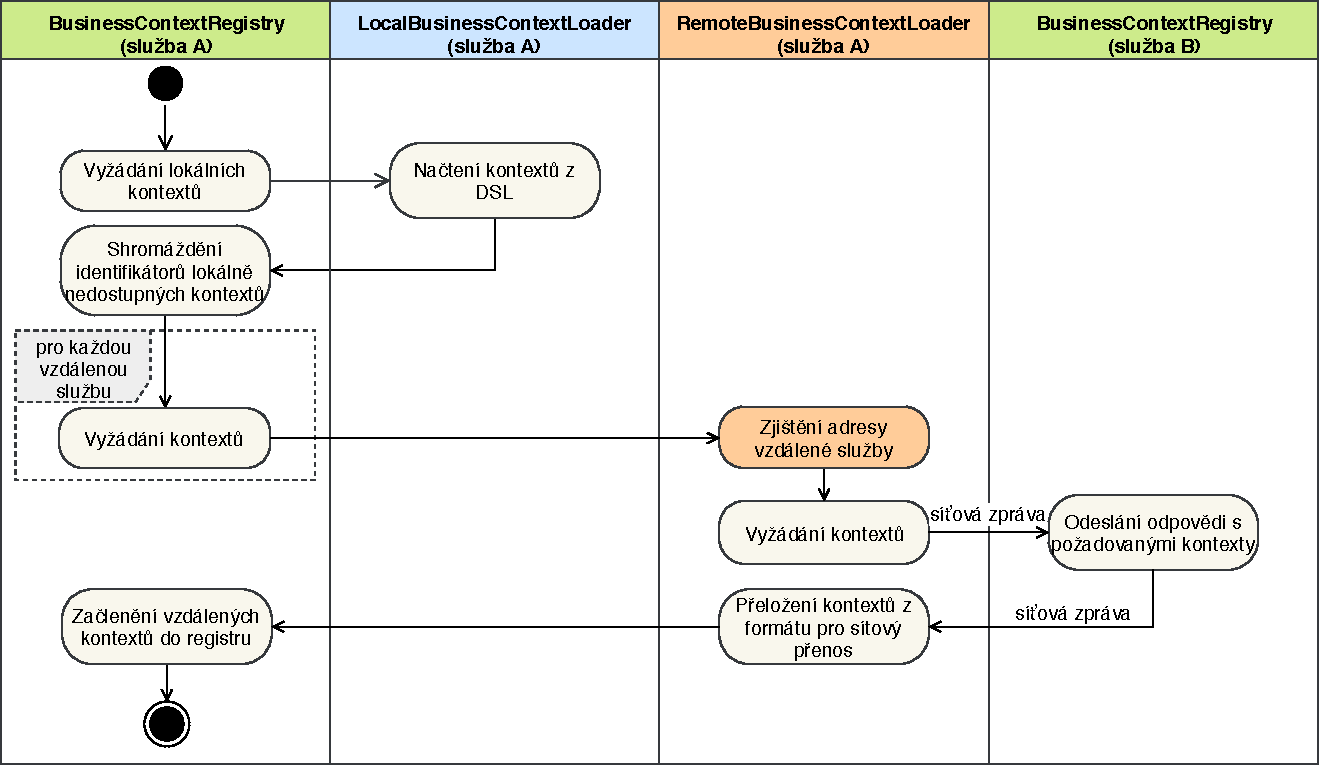
\includegraphics[keepaspectratio=true, width=\linewidth]{figures/business-context-loading.pdf}
    \caption{Diagram procesu inicializace byznysov\'ych kontextů}
    \label{fig:business-context-loading}
\end{figure}

Během inicializiace byzynsových kontextů je potřeba nejprve načíst lokálně dostupné kontexty popsané pomocí \gls{DSL}.
Po převedení z \gls{DSL} do metamodelu je potřeba shromáždit seznam rozšířených kontextů a zjistit, které
rozšířené kontexty nejsou lokálně dostupné. Následně je potřeba vyžádat si vzdálené kontexty od příslušných služeb
a převést obdržené kontexty z formátu pro síťový přenos do formátu, ve kterém budou kontexty uloženy v paměti.
Nakonec je potřeba, aby do všech kontextů, které využívají dědičnosti, byly začleněny byznysová pravidla
rozšířených kontextů. Celou inicializaci může zastřešovat komponenta \code{BusinessContextRegistry}, která
je vhodným kandidátem, protože má znalost o všech subsystémech, které jsou k tomuto procesu potřeba.
Jak si můžeme všimnout, tato komponenta implementuje návrhový vzor \textit{Facade}~\cite{fowler2002patterns}.
Na obrázku~\ref{fig:business-context-loading} je znázorněn navržený proces inicializace.

\section{Centráln\'{\i} správa byznys kontextů}

Vzhledem k nutnosti centralizovat správu byznysových kontextů se nám
architektura \gls{P2P} představená v subsekci~\ref{sec:p2p} nehodí.
Při úpravě kotextů by totiž v systému mohly existovat staré i nové verze
byznysových pravidel, což je pro správnou funkci systém nepřijatelné.
Využijeme tedy architektury klient-server s více servery.
Byznysové kontexty budou podle svého prefixu rozděleny do skupin
a každou ze skupin bude spravovat jedna služba, která bude zároveň
držet jejich aktuální a jediný stav.

\subsection{Uložen\'{\i} rozšířeného pravidla}\label{sec:saving-context}

\goal{Diskutovat chaining vs. direct update}
Při ukládání byznysového kontextu, od kterého dědí jiné kontexty, musíme zajistit, že
bude změna korektně propagována. Máme dva způsoby, kterými toho můžeme docílit. Jeden z nich je,
že služba, která je původcem upraveného pravidla, sama informuje o změně všechny ostatní služby,
které si od ní pravidlo vyžádaly. Tento způsob však vyžaduje implementaci registru, do kterého by
si služba poznamenávala které služby při změně kterého pravidla kontaktovat. Navíc není zaručeno,
že to vždy půjde, protože služba teoreticky nemusí být v opačném směru dostupná \textendash\xspace například
kvůli překladu síťových adres \gls{NAT}.

Druhým způsobem je přenechat kontaktování zúčastněných služeb na nástroji pro centrální
správu byzynsových pravidel. Ten má totiž přehled o všech závislostech v systému a zároveň
zná i adresu všech služeb. Nástroj by tak mohl při ukládání upraveného pravidla zmapovat,
které kontexty je potřeba aktualizovat, a následně požádat služby, ke kterým kontexty patří,
aby tyto kontexty znovu sestavili. Nevýhodou tohoto přístupu je zvýšená komunikačmní zátěž kvůli většímu
objemu přenesených informací. V tuto chvíli lze spekulovat, že tato zátěž je vůči absolutnímu objemu
přenášených dat v systému využívajícímu \gls{SOA} zanedbatelná. Bylo by ale vhodné při implementaci
vybrat vhodný přenosový formát, který minimalizuje dopad veškeré síťové komunikace týkající se
byznysových pravidel.

\subsection{Proces úpravy kontextu}

\begin{figure}
    \centering
    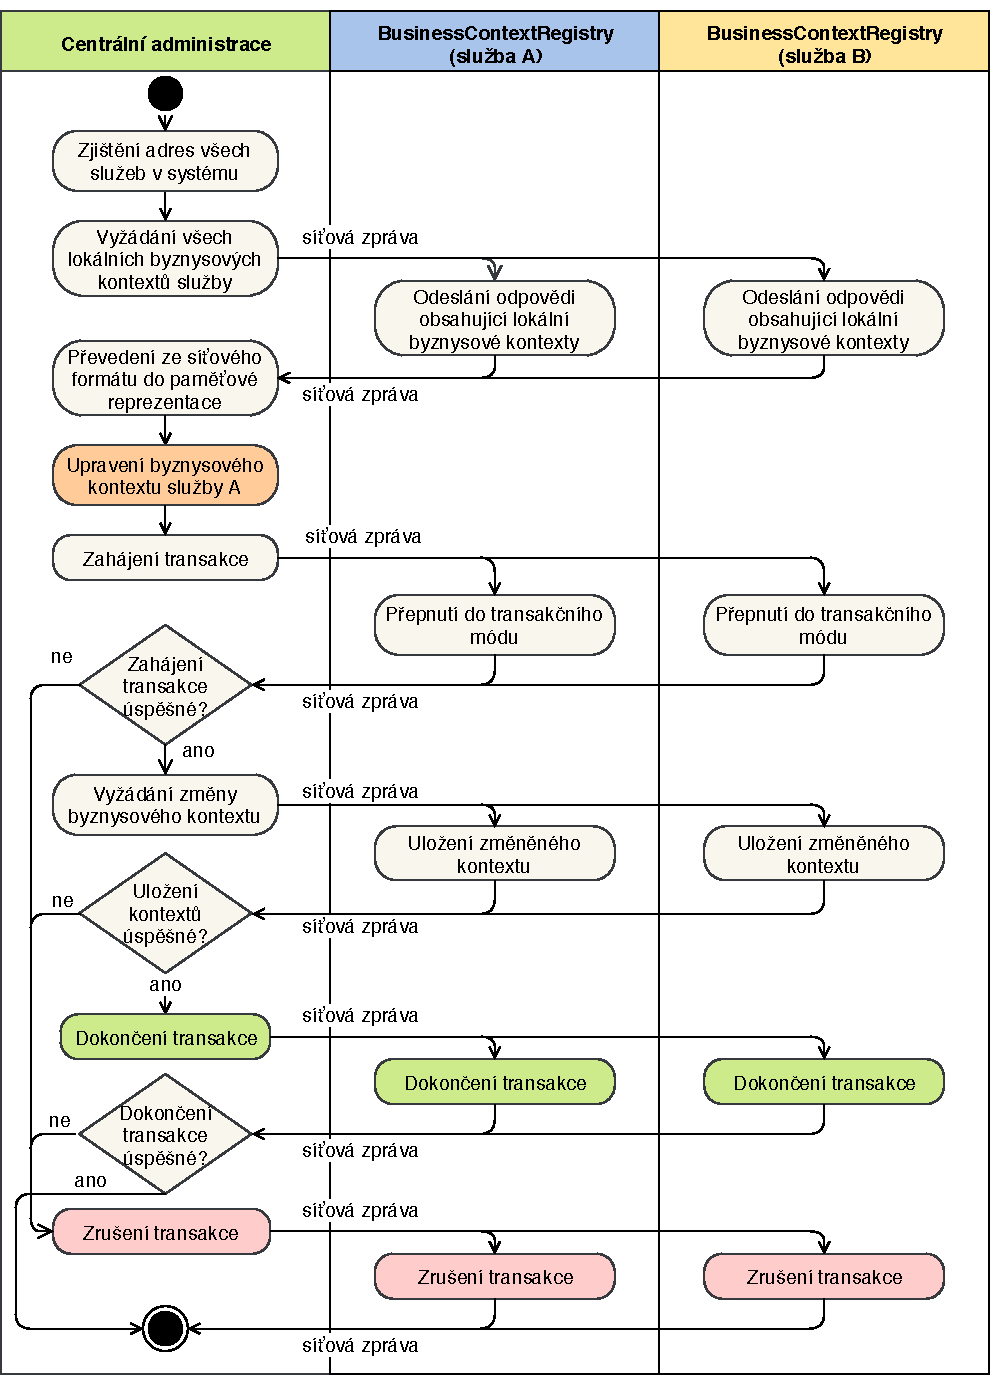
\includegraphics[keepaspectratio=true, width=\linewidth]{figures/business-context-management.pdf}
    \caption{Diagram procesu centráln\'{\i} správy byznysov\'ych kontextů}
    \label{fig:business-context-management}
\end{figure}

Nyní můžeme navrhnout samotný proces úpravy byznysového kontextu pomocí nástroje pro
centrální administraci. Ten pro svou funkci musí načíst všechny byznysové kontexty všech
služeb v systému. Následně může zobrazit administrátorovi formulář pro úpravu pravidla.
Pravidlo by mělo být převedeno z metamodelu do \gls{DSL} pro snažší úpravu.
Po odeslání formuláře bude pravidlo převedeno zpět do metamodelu.
Nástroj pro administraci by měl v tuto chvíli analyzovat na které služby bude
mít změna pravidla dopad. Následně je s těmito službami zahájena transakce, při které v nich
nesmí probíhat žádná byznysová operace. Když všechny ovlivněné služby zahájí transakci, je možno
jim rozeslat novou podobu pravidla. Pokud vše proběhne v pořádku, je možno transakci dokončit
a služby otevřít byznysovým transakcím. Pokud naopak některý z kroků transakce selže, je nutno
informovat všechny zúčastněné služby o zrušení transakce a změnu inkriminovaného pravidla zrušit.
Na obrázku~\ref{fig:business-context-management} je celý proces znázorněn. Proces pro uložení nového kontextu je analogický.

\section{Architektura frameworku}\label{sec:architecture}

Nyní, když jsme navrhli jednotlivé části systému a jejich součinnost, můžeme popsat
architekturu celého frameworku. V této sekci budeme předpokládat klasickou třívrstvou
architekturu~\cite{fowler2002patterns}, která se skládá z prezentační, aplikační a datové vrstvy.
Každá z těchto vrstev může využívat náš framework \textendash\xspace prezentační vrstva
při validování vstupních polí formuláře, aplikační vrstva při aplikaci byzynsových pravidel
v byznysových operacích a datová vrstva při aplikaci post-conditions pro filtrování dat
při jejich získávání z databáze. Pro účely této práce se soustředíme zejména na aplikaci
v aplikační vrstvě.

\begin{figure}
    \centering
    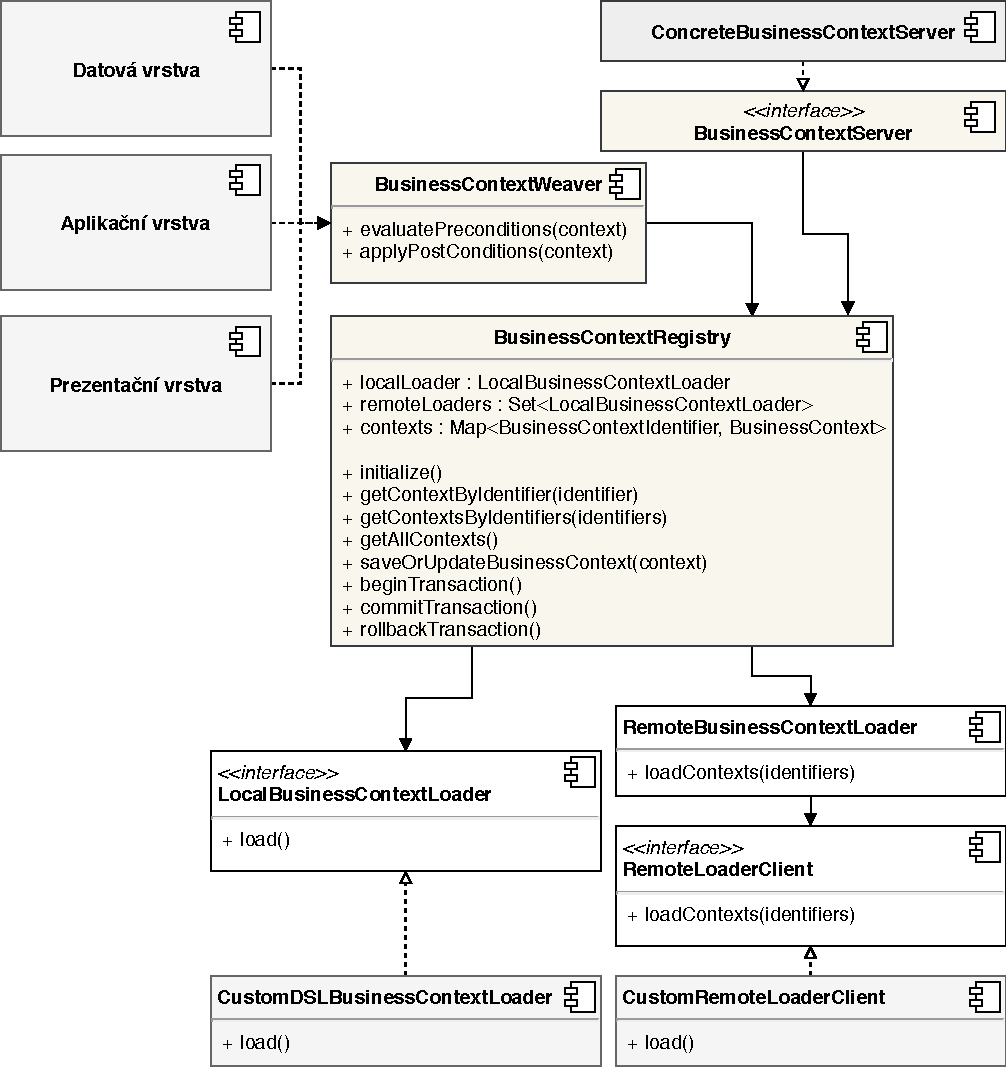
\includegraphics[keepaspectratio=true, width=\linewidth]{figures/business-context-registry.pdf}
    \caption{Diagram tříd navrženého frameworku}
    \label{fig:business-context-registry}
\end{figure}

Středobodem našeho frameworku je komponenta \code{BusinessContextRegistry}, tedy registr
byznysových kontextů, který je zodpovědný za inicializaci a uchovávání byznysových kontextů.
Načítání lze rozdělit na lokální a vzdálené. Při načítání lokálně dostupných kontextů
je potřeba získat \gls{DSL} kontextu ze souboru či databáze a převést ho do metamodelu.
K tomu bude využito rozhraní \code{LocalBusinessContextLoader}. Implementace rozhraní může být libovolná
a záviset na použitém \gls{DSL} či místu uložení pravidel. Naopak při načítání vzdálených
kontextů je potřeba vyžádat kontexty od vzdálené služby. O to se postará třída \code{RemoteBusinessContextLoader},
která požadované kontexty zoraginzuje podle prefixu a poté pomocí rozhraní \code{RemoteLoaderClient} načte
pravidla od jednotlivých služeb. Implementace rozhraní \code{RemoteLoaderClient} bude záviset na použité
technologii a zajistí síťovou komunikaci a převod do a z formátu pro síťový přenos.

Aby mohl framework poskytovat lokální byznysové kontexty dané služby ke stažení, musí zastřešit
i serverovou funkcionalitu. K tomu slouží rozhraní \code{BusinessContextServer}. To bude využívat
\code{BusinessContextRegistry}, ze kterého načte byznysové kontexty, které si vyžádá \code{RemoteLoaderClient}.
Implementace serveru bude opět závislá na konkrétní technologii.

Nakonec bude framework obsahovat sadu aspect weaverů, které umožní weaving byznysových pravidel do
jednotlivých vrstev systému. Pro účely této práce poskytneme weavery pro využití v aplikační vrstvě
pro weaving preconditions a post-conditions do byznysových operací.

\subsection{Service discovery}

Abychom mohli přenášet byznysové kontexty mezi službami, musí služba vyžadující kontext
znát adresu služby, od které ho vyžaduje. Adresy služeb mohou podléhat různým konfiguracím,
které se mohou lišit systém od systému. Náš framework proto nesmí být závislý na způsobu,
jakým se adresování služeb provádí. Nejlepším způsob je přenechat na uživateli, aby sám
frameworku předal adresy služeb ve chvíli, kdy je framework potřebuje \textendash\xspace tedy
ve chvíli, kdy je potřeba načíst lokálně nedostupné kontexty.

\section{Shrnutí}

V této kapitole jsme navrhli framework pro centrální správu a automatickou distribuci
byznysových pravidel v \gls{SOA} na základě přístupu \gls{ADDA}. Formalizovali jsme
doménu \gls{SOA} do názvosloví \gls{AOP}. Diskutovali jsme podobu byznysových pravidel a jejich
logických výrazů a jakým způsobem ji zachytit jak v paměti počítače, tak pomocí \gls{DSL}.
Zvážili jsme výhody organizace pravidel do byznysových kontextů a představili koncept dědičnosti.
Vymodelovali jsme procesy, kterými budou pravidla distribuována a také proces pro přídání či úpravu
byznysového pravidla za běhu systému. Nakonec jsme shrnuli celkovou architekturu frameworku.
